%%%%%%%%%%%%%%%%%%
%%%   Template para utilização   %%%
%%%%%%%%%%%%%%%%%%

%Para melhor utilização da ferramenta, utilize o pdfLaTeX+MakeIndex+BibTeX%

\documentclass[12pt,openright,oneside,a4paper,english,spanish,brazil]{unifil}
%%\usepackage{algorithm,algpseudocode}
\usepackage[portuguese, ruled, linesnumbered]{algorithm2e}
\usepackage{graphicx}
\graphicspath{figuras/}


\titulo{Detecção de Anomalias em Redes: Taxonomia de técnicas e um Estudo de Caso%Adicionar título da sua monografia%
}
\autor{Bruno Prece da Silva%Adicionar seu nome%
}
\instituicao{Centro Universitário Filadélfia
}
\local{Londrina
}
\data{2016%Adicionar o ano de publicação%
}
\preambulo{Ciência da Computação%Adicionar seu curso%
}
\orientador{Me. Mario Henrique Akihiko da Costa Adaniya%Adicionar seu orientador
}

\begin{document}

\frenchspacing

%%%%%%%%%%%%%%%%%%%%%%%%%
%%%%%%Elementos pré-textuais%%%%%%%%%
%%%%%%%%%%%%%%%%%%%%%%%%%

\pretextual

%Capa%

\imprimircapa

%Folha de Rosto%

\makeatletter
\renewcommand{\folhaderostocontent}{
\begin{center}
{\ABNTEXchapterfont\bfseries\MakeTextUppercase{\imprimirautor}}
\vspace*{5cm}
\begin{center}
\ABNTEXchapterfont\bfseries\normalsize\MakeTextUppercase{\imprimirtitulo}
\end{center}
\vspace*{1cm}
\abntex@ifnotempty{\imprimirpreambulo}{%
\hspace{.45\textwidth}
\begin{minipage}{.5\textwidth}
\SingleSpacing
 Trabalho de Dissertação apresentado ao \imprimirinstituicao como parte dos requisitos para obtenção de graduação em \imprimirpreambulo.
{\textnormal{\imprimirorientadorRotulo~\imprimirorientador.}}
\end{minipage}%
}%
\vspace*{\fill}
{\bfseries\large\imprimirlocal}
\par
{\bfseries\large\imprimirdata}
\vspace*{1cm}
\end{center}
}
\makeatother

\imprimirfolhaderosto

\clearpage{\pagestyle{empty}\cleardoublepage}

%Folha de Aprovação%

\begin{folhadeaprovacao}
	\begin{center}
		\ABNTEXchapterfont\textbf{\MakeTextUppercase{\imprimirautor}}
		\vspace*{2cm}
		\begin{center}
			\ABNTEXchapterfont\large\textbf{\MakeTextUppercase{\imprimirtitulo}}
		\end{center}
		\vspace*{2cm}
		Trabalho de Conclusão de Curso apresentado à Banca Examinadora do curso de \imprimirpreambulo do \imprimirinstituicao de \imprimirlocal em cumprimento a requisito parcial para obtenção do título de Bacharel em \imprimirpreambulo.
		\par
		\vspace*{.5in}
		\hspace{.6\textwidth}
		\begin{minipage}{.6\textwidth}
			\begin{center}
\MakeTextUppercase{Aprovado pela \textbf{COMISSÃO EXAMINADORA} em \imprimirlocal, \imprimirdata.}
			\end{center}
		\end{minipage}
			\vspace*{\fill}
			\assinatura{{\imprimirorientador} - Orientador}
			\assinatura{Professor 1 - Examinador} %Insira o nome dos outros examinadores
			\assinatura{Professor 2 - Examinador} 
	\end{center}
\end{folhadeaprovacao}

%Dedicatória (opcional)%

\begin{epigrafe}
\vspace*{\fill}
\begin{flushright}
%%
Este trabalho é dedicado aos que acreditam em pôneis mágicos...
\end{flushright}
\end{epigrafe}

%Agradecimentos (opcional)%

\begin{agradecimentos}

%%Insira seus agradecimentos
Agradeço a Deus, minha família, amigos, professores e ao Centro Universitário Fildélfia pela optortunidade concedida através da bolsa.
\end{agradecimentos}

%Epígrafe (opcional)%

%%Insira sua epígrafe entre as chaves do \textit{}

\begin{epigrafe}
\vspace*{\fill}
\begin{flushright}
\textit{"Eu sou o caminho, e a verdade e a vida; ninguém vem ao Pai, senão por mim." \\
(João 14:6)}
\end{flushright}
\end{epigrafe}

% --- resumo em português ---
	%%Altere as informações do resumo%%
\noindent{SILVA; Bruno Prece, \textbf{\imprimirtitulo}. Trabalho de Conclusão de Curso (Graduação) - \imprimirinstituicao. \imprimirlocal, \imprimirdata.}
\par
\begin{resumo}
	%%Escreva seu resumo na língua vernácula aqui%%
Resumo em português.
\vspace{\onelineskip} \\
	%%Adicione as palavras chaves após os dois pontos '':''%%
\noindent
\textbf{Palavras-chaves}: Detecção de Anomalias, clustering, segurança da informação.
\end{resumo}

% --- resumo em inglês ---
	%%Altere as informações do resumo%%
\noindent{SILVA; Bruno Prece. \textbf{\imprimirtitulo}. Trabalho de Conclusão de Curso (Graduação) - \imprimirinstituicao. \imprimirlocal, \imprimirdata.}
\par
	%%Se o seu resumo não for em inglês, altere o ``Abstract'' e ``english'' abaixo.
\begin{resumo}[Abstract]
\begin{otherlanguage*}{english}
	%%Write your abstract in foreign language here%%
\emph{
Extended abstract in English or another foreign language. 30 lines, simple spacing.
}
\vspace{\onelineskip}
\noindent
	%%Add the keywords after the colon '':''%%
\emph{	
\textbf{Keywords}: Detecção de Anomalias, clustering, segurança da informação.}
\end{otherlanguage*}
\end{resumo}

%\par
%\vspace{11cm}

\tableofcontents*

  \setlength\absleftindent{0cm}
  \setlength\absrightindent{0cm}
  
  %fonte do ambiente%
  \abstracttextfont{\normalfont\normalsize}

  %intentação e espaçamento entre parágrafos%
  \setlength{\absparindent}{0pt}
  \setlength{\absparsep}{18pt}

%\pdfbookmark[0]{\listfigurename}{lof}
%\listoffigures*
%\cleardoublepage

\textual

\renewcommand{\ABNTEXchapterfont}{\fontfamily{cmr}\fontseries{b}\selectfont}
\renewcommand{\ABNTEXchapterfontsize}{\Large}

\renewcommand{\ABNTEXsectionfont}{\uppercase{\fontfamily{cmr}\fontseries{b}\selectfont}}
\renewcommand{\ABNTEXsectionfontsize}{\large}

\chapter{Introdução}%%Inserir título do capítulo (nível 1)
\indent A constante expansão na utilização da Internet tornou a rede um serviço essencial para a interconexão global e para as empresas. A cada dia há um crescimento na demanda por  novos serviços, que necessitam de políticas de segurança que mantenham a integridade e a privacidade dos dados. Isso torna os sistemas cada vez mais complexos e os dados cada vez mais heterogêneos, impossibilitando que a gerência da rede seja realizada por um operador humano. Devido à esta dificuldade de gerência, surgem comportamentos que fogem dos padrões normais do tráfego, estes comportamentos são as anomalias. Uma anomalia pode ser definida como uma não conformidade com o comportamento normal de uma determinada base de dados.

\indent As anomalias podem ser geradas por vários fatores, podendo ser maliciosas, como, por exemplo, ataques de negação de serviço (\textit{Dos}), exércitos de máquinas controladas sem autorização (\textit{botnets}) e envio massivo de correio eletrônico (\textit{spam}). E podem não ser maliciosas, como, interrupções não planejadas, crescimento repentino de tráfego, e tráfego de uma única fonte para muitos destinos. Deste modo, os \textit{firewalls} não são suficientes para manter segurança e integridade dos sistemas, pois, não conseguem evitar ataques externos. Já os sistemas de autenticação, não conseguem evitar um comportamento nocivo de um usuário legítimo, além disso, estes sistemas possuem limitações para verificar anomalias causadas pela utilização não nociva e por problemas nos equipamentos.

\indent A detecção de anomalias em redes é uma tarefa extremamente difícil, principalmente porque as anomalias são alvos móveis presentes em um conjunto de dados heterogêneos, que dificulta a precisão em encontrar um determinado conjunto de dados do tráfego que caracterizam uma anomalia. Além disso, para classificar uma anomalia é necessário conhecer o seu perfil, e a dificuldade desta tarefa aumenta a cada dia com o surgimento de novos tipos ataques e técnicas de invasão.

\indent De maneira geral, os estudos classificam a detecção de anomalias em duas vertentes, baseada no comportamento normal da rede, onde busca-se caracterizar um perfil do tráfego normal, e a cada novo evento é realizada uma comparação com o perfil normal, caso o evento não se enquadre, será considerado um comportamento anômalo. E na detecção baseada em assinaturas, será implementado um banco de dados com o perfil de várias anomalias, e assim, cada evento do tráfego será confrontado com estes perfis anômalos, a fim de verificar se o evento capturado possuí características semelhantes às anomalias. 

\indent O objetivo deste trabalho é apresentar os principais métodos de detecção de anomalias presentes na literatura, trazer análises referentes às vantagens e desvantagens de cada abordagem e os tipo de dados em que apresentam maior eficaz. Além disso, apresentamos um estudo de caso utilizando a técnica de clusterização dos dados, uma abordagem simplificada, muito explorada na literatura e apresenta bons resultados.

\chapter{Fundamentação Teórica}

  \section{Anomalias}

\indent Uma anomalia é caracterizada por um desvio do padrão normal de uma determinada base de dados. As técnicas para detecção de anomalias ou, também chamadas de outliers, vêm sendo estudadas pela comunidade estatística desde o fim do século 19 (EDGEWORTH, 1887), diversas técnicas foram estudadas e produzidas, algumas para bases de dados específicas, enquanto outras são genéricas.

\indent No tráfego de rede as anomalias representam ações que se diferem do comportamento normal que já foi analisado. Mesmo quando uma anomalia não impacta profundamente a rede, ela atinge a qualidade dos serviços que são entregues aos usuários finais (LAKHINA et al., 2004).  Este comportamento anômalo pode representar eventos de origem maliciosa e não maliciosa, que irão afetar a rede de diversos modos. 

  \indent Anomalias de origem maliciosa são geradas por um atacante humano que tem por objetivo afetar o serviço de rede entregue aos usuários, ou conseguir acesso a dados privados. É o tipo de anomalia mais prejudicial, onde, uma invasão, por exemplo, pode ocasionar o compromentimento total da rede e o acesso a dados sigilosos que certamente afetará seus usuários e a empresa ou instituição responsável pela rede.
  \begin{itemize} 
  \item \textbf{Ataque de negação de serviço:} também conhecido como DoS \textit{(Denial of Service)} é um ataque que consiste em uma tentativa de tornar indisponíveis os recursos de uma vítima. Neste tipo de ataque não ocorrem invasões, nem tentativas de se apropriar de dados sigilosos. Um ataque DoS de fontes maliciosas envia uma enorme quantidade de pacotes para a vítima, fazendo com que esta sobrecarga  torne a vítima inoperável ao não conseguir atender à todas solicitações. Uma variação deste ataque é o DDoS \textit{(Distributed Denial of Service)}, um ataque mais elaborado, onde um atacante controla diversas máquinas zumbis que atacam a vítima. Este ataque possui uma hierarquia de máquinas, assim, as próprias máquinas zumbis podem controlar outras máquinas. Geralmente este ataque tem a duração de vinte minutos (LAKHINA et al., 2004).
  \item \textbf{Varredura de portas:} o \textit{scanner} de portas é uma atividade que tem como objetivo encontrar vulnerabilidades em uma aplicação. Na varredura de portas há uma máquina que envia pacotes de testes em direção às portas da vítima, conseguindo detectar quais serviços estão ativos em cada porta. Esta atividade ocasiona um aumento no tráfego de pacotes, além disso, se caracteriza por não possuir uma relação dominante entre um IP de origem e uma porta de destino. 
  \item \textbf{\textit{Worms:}} são programas de códigos maliciosos que se propagam na rede, a fim de encontrar vulnerabilidades, conseguir acesso a dados sigilosos e infectar outras máquinas. Um \textit{worm} se replica rapidamente na rede ameaçando toda a infraestrutura devido ao grande aumento no tráfego, onde as máquinas infectadas enviam pacotes aleatoriamente para outros alvos. Alguns \textit{worms} são tão sofisticados que conseguem esconder suas atividades de muitos IDS (\textit{Intrusion Detection Systems}) (MONOWAR et al., 2014), podendo ficar por vários dias sem se manifestar na rede até que sejam acionados por um usuário ou se acionarem automaticamente em um situação específica.
  \item \textbf{Ataques de Penetração:} há dois tipos principais de ataques de penetração, o ataque R2L (\textit{Remote to Local}) que ocorre quando um usuário consegue acesso a uma máquina remotamente. O atacante envia pacotes para uma máquina alvo e analisa e explora sua vulnerabilidades para ganhar acesso. O ataque U2R (\textit{User to Root}) se baseia em um atacante que possui acesso em um sistema, e ao explorar sua vulnerabilidades consegue acesso como administrador (SILVA, 2007). Estes tipos de ataques têm como objetivo usufruir dos recursos e dados de um sistema, podendo prejudicar toda a rede.
  \item \textbf{\textit{Spam}:} De acordo com (FEITOSA, 2008), o \textit{spam} pode ser definido com um envio massivo de correio eletrônico a um grande número de usuários. Essas mensagens podem ser classificadas de acordo com o conteúdo, podendo conter propagandas, códigos maliciosos, páginas de \textit{phishing} e golpes. Este ataque é direcionado a servidores SMTP (\textit{Simple Mail Transfer Protocol}) responsáveis pelo envio de correio eletrônico. São criadas inundações de \textit{e-mails} no servidor e utilizam de forma inadequada a banda que seria utilizada pelos usuários legítimos.
  \end{itemize}  


\indent Segundo (SILVA, 2007), as anomalias de origem não maliciosas são geradas por  aumentos repentinos de tráfego e por eventos de falhas na rede, que incluem, problemas de configuração, interrupções de funcionamento e até mesmo uma adição imperfeita de novos dispositivos.

\begin{itemize}
  \item \textbf{\textit{Flash crowd:}} pode ser definido como uma grande demanda por serviço ou recurso da rede. Consiste basicamente no aumento repentino de clientes que de maneira não organizada enviam requisições a um servidor. Esta sobrecarga, apesar de não ser maliciosa atua como um \textit{DoS}, podendo deixar a rede inoperável. Um exemplo de \textit{flash crowd} ocorre quando são lançadas atualizações para as distribuições Linux, a quantidade de usuários solicitando recursos dos repositórios FTPs acaba deixando o serviço inoperável por um certo tempo.
  \item \textbf{\textit{Alpha Flows:}} Fluxos \textit{Alpha} são resultados do aumento no volume do tráfego entre uma relação de IP de origem e porta destino, ocasionado por uma grande quantidade de transferência de arquivos ou experimentos em uma rede.
  \item \textbf{\textit{Broadcast} Storms:} Tempestades de \textit{broadcast} podem ocorrer devido a falhas de software e configuração nos nós da rede. Geralmente utilizado pelo protocolo ARP para encontrar os endereços físicos dos \textit{hosts} da rede, os pacotes \textit{broadcast} são enviados a todos \textit{hosts}, para que a máquina buscada informe seu endereço físico para o roteador ou \textit{switch}. Uma grande quantidade de pacotes \textit{broadcast}  pode causar interrupções e congestionamentos na rede, afetando o serviço entregue aos usuários finais. Este tipo de anomalia também é comum em redes com impressoras sem fio, onde os \textit{softwares} de controle da impressora disparam tempestades de \textit{broadcast} na rede em busca da impressora caso ela seja removida.
  \item \textbf{\textit{Babbling node:}} ocorre quando um nó da rede, por alguma falha, começa a enviar pacotes aleatoriamente na rede, segundo (AL-KASASSBEH; ADDA, 2009) estas anomalias ocorrem com as placas de rede, que começam a enviar pacotes de controle aleatoriamente.
  \item \textbf{Erros de configuração em \textit{firewalls:}} a configuração de um dispositivo de \textit{firewall} pode bloquear pacotes que estão entrando na rede, com isso, surgem mudanças repentinas no tráfego (Zarpelão, 2009). Além disso, podem surgir congestionamentos devido a grande quantidade de bloqueios do \textit{firewall} em um curto espaço de tempo.
  \item \textbf{Congestionamentos:} é a principal consequência gerada pelas anomalias, basicamente, um congestionamento ocorre com um aumento significativo do tráfego em um ponto da rede, o que causa problemas para o processamento dos pacotes, ocasionando demora para a entrega dos pacotes, ou até mesmo o descarte caso o seu TTL (\textit{Time To Life}) se esgote ou o nó da rede o corrompa.
\end{itemize}


  \section{Classificação de Técnicas de Detecção}


\indent As principais vertentes de pesquisas dividem as técnicas de detecção de anomalias em detecção baseada em assinaturas de anomalias e detecção baseada na caracterização do comportamento normal da rede. Na detecção baseada em assinatura é necessário a criação de uma base de dados que contenham essas assinaturas, para isso, um analista humano necessita analisar extensas bases de dados \textit{post-mortem} para encontrar padrões já catalogados de comportamentos que caracterizam anomalias (SILVA, 2007). Assim, com a base de dados criada, os dados da rede são coletados e os eventos reais são comparados às assinaturas. Caso o evento do tráfego real se enquadre em uma assinatura uma notificação é gerada.

\indent Em relação às vantagens da detecção baseada em assinatura, destaca-se sua precisão na detecção de anomalias já conhecidas, além disso, a técnica possui baixa taxa de falsos positivos, onde eventos não anômalos são classificados como anomalias. As desvantagens desta técnica se dão principalmente pela incapacidade de detectar anomalias que não estão catalogadas, que surgem constantemente com o crescimento das redes e desenvolvimento tecnológico (ZARPELÃO, 2009). Além disso, esta técnica necessita de revisões constantes na base de dado para inserção de novas assinaturas.

\indent A detecção baseada no comportamento normal consiste na criação de um perfil de normalidade da rede, onde os dados do tráfego são analisados por semanas ou meses até que se possa caracterizar o perfil normal da rede em cada instante do dia e de cada dia da semana. Deste modo, novos eventos são comparados com o perfil correspondente ao instante em que o evento foi coletado, se o desvio do evento em relação ao perfil normal ultrapassar limites previamente definidos, o evento é classificado como uma anomalia.

\indent Esta abordagem é muito eficaz na detecção de anomalias conhecidas e desconhecidas, porém muitos desafios surgem para a implementação desta técnica. Primeiramente há grande dificuldade na caracterização do perfil normal da rede, onde, por exemplo, se uma anomalia é constante na rede durante a coleta de tráfego para a caracterização do perfil normal, essa anomalia terá influencia no perfil e anomalias semelhantes não serão detectadas. Um desafio para os pesquisadores é a diminuição das taxas de falsos positivos gerados, que está relacionada aos limites de desvio definidos na implementação. Quanto maior o limite, menos alarmes falsos são gerados, pois é maior a tolerância de desvio entre o evento capturado e o perfil normal. Já, quanto menor o limite estreita-se mais a tolerância desde desvio, assim, eventos que não caraterizam anomalias podem ser considerados anômalos, por exemplo, um aumento no tráfego legítimo em um período onde os perfis caracterizam um tráfego baixo.

\indent A rotulagem de dados utilizada nas abordagens também é utilizada para a classificação das técnicas. Como já visto, alguns sistemas utilizam a assinatura da anomalia enquanto outros optam pela a assinatura do comportamento normal. Mas há sistemas híbridos que mesclam as duas rotulagens e sistemas que não utilizam nenhum tipo de assinatura.

\indent Sistemas de detecção supervisionados utilizam tanto a classe de assinatura de anomalias quanto a classe de assinatura do perfil normal do tráfego. O sistema compara cada evento gerado com as duas classes, assim, classifica o evento capturado em relação à classe em que mais se enquadra (CHANDOLA et al., 2009). Este tipo de abordagem irá enfrentar os problemas para a rotulagem das duas classes de dados, além de caracterizar o tráfego normal, terá de realizar revisões constantes na base de assinaturas anômalas para inserção de novas assinaturas. Torna-se redundante utilizar os dois modos de rotulagem, já que os eventos anômalos ocorrem em quantidade muito menor em relação aos eventos normais (MONOWAR et al., 2014). 
 
\indent Um sistema semi-supervisionado leva em consideração a sua implementação apenas os dados rotulados do perfil normal do tráfego. Não necessitando das assinaturas de anomalias, um sistema semi-supervisionado pode ser implementado mais facilmente em relação aos sistemas supervisionados. Para diminuir a influência de anomalias no processo de caracterização do tráfego normal, alguns trabalhos como (LUCENA et al., 2009) realizam análises no tráfego coletado para utilizar dados que não apresentam indícios de anomalias que afetam a rede em grande escala.    
    
\indent As abordagens não supervisionadas não utilizam nenhum tipo de assinatura, assim, são mais fáceis de ser aplicadas na rede, mas são difíceis de implementar. Geralmente estes sistemas buscam analisar as relações do fluxo de rede e o conteúdo dos pacotes e partir destes dados utilizam outras técnicas, como, clusterização, outliers e redes neurais para encontrar e caracterizar as anomalias. Alguns trabalhos, como (MAZEL et al., 2015) implementam sistemas não supervisionados, no caso, para detectar anomalias são analisados mudanças na média de variância no fluxo da rede, capturando esses eventos e realizando a clusterização dos dados em grupos que compõem anomalias e um grupo de tráfego normal.
    
  
  \section{Algoritmos Estatísticos}
\indent Nos métodos baseados em estatística, é criado um perfil do comportamento da rede à partir do momento em que o tráfego começa a ser coletado. Este perfil leva em consideração as características do tráfego, como número de pacotes por protocolo de rede, quantidade de protocolos, número de conexões, entre outros (PERLIN et al., 2011). A partir destes dados, um limiar fixo ou dinâmico é estabelecido, ou seja, um limite é criado para avaliar a variação dos eventos capturados naquele momento em relação ao perfil gerado por eventos capturados anteriormente.

\indent A principal vantagem na utilização de algoritmos estatísticos se dá por esta técnica não necessitar de uma etapa de treinamento para geração de um perfil normal. Os sistemas possuem a capacidade de aprender o comportamento esperado da rede, pois, o perfil é criado durante a própria análise do tráfego (TEODORO et al., 2008). Este perfil obedece a variabilidade constante da rede, sendo assim, um crescimento gradual do tráfego que não representa uma anomalia, não será classificado como anômalo simplesmente por ultrapassar os limites definidos, como pode ocorrer em abordagens que utilizam dados de treinamento. 

\indent No entanto, há grandes dificuldades para implementação de sistemas com algoritmos estatísticos. Primeiramente, ataques podem ser feitos à rede de tal maneira que o tráfego gerado pode ser considerado normal por não afetar o tráfego de maneira brusca. Em segundo lugar, a escolha pelo tipo de algoritmo estatístico ideal não é uma tarefa fácil (CHANDOLA et. al, 2009), além disso, há dificuldade de definir limiares que mantenham o equilíbrio entre as taxas de detecção e a quantidade de falsos positivos e falsos negativos.

%% HÁ DOIS TRABALHOS DE WANG EM 2009, OS DOIS SÃO CITADOS NO PARÁGRAFO.
\indent Em (LUCENA et al., 2009) o algoritmo de Holt-Winters juntamente com medidas de entropia são utilizados para detecção de anomalias em redes WAN. Nos trabalhos de WANG et al (2009) e SAMAAN et al (2008) são utilizados modelos autorregressivos (AR) para a previsão do tráfego. O trabalho de SILVA (2003) baseia-se na utilização de cálculos de média e desvio padrão para detecção de intrusões nas redes e em WANG et al (2009) são abordados funções ARMA para análise de autocorrelação nos dados da rede. 

\indent Um dos algoritmos estatísticos amplamente abordados na literatura é a Transformada Wavelet, um método matemático de análise multiescalar capaz de decompor um sinal em diferentes níveis para análise. Cada nível da transformada contém informações e variações complementares ao nível médio, também denominado nível grosseiro, que representa as informações em relação a média do comportamento do sinal (PERLIN et al., 2011). A Transformada de Wavelet Discreta é uma variação da Transforma de Wavelet implementada pelo Algoritmo Piramidal de Mallat (MALLAT, 1998), este algoritmo utiliza filtros para o processamento dos sinais, gerando coeficientes de aproximação e coeficientes de detalhes. Os coeficientes de aproximação representam a média ponderada dos sinais, enquanto os de detalhes apresentam informações complementares e detalhes que não se enquadram na média ponderada (RIGHI et al., 2014).

\indent Na detecção de anomalias a Transformada de Wavelet consegue diminuir ou eliminar a correlação, assim, anomalias de curta duração podem ser detectadas com mais precisão em modelos que utilizam trechos curtos de tráfego durante a análise, além disso, a decomposição dos sinais possibilita o isolamento de mudanças bruscas em longos trechos de tráfego. Deste modo, a Transformada de Wavelet possibilita a detecção de anomalias independente da duração do tráfego analisado (WANG et al., 2009).
    
  \section{Redes Neurais}
\indent As Redes Neurais foram desenvolvidas com base no modo que o cérebro humano organiza os neurônios ao executar cálculos relacionados ao reconhecimento de padrões, controle motor e percepção (MONOWAR et al., 2014). As Redes Neurais têm sido empregadas em diversos tipos de aplicações que visam um bom desempenho em tomadas de decisões. A principal aplicação das redes neurais se dá na resolução de problemas que dependem do reconhecimento de padrões, classificação e aproximação de dados. 

\indent O reconhecimento de padrões em certas bases de dados pode ocorrer de forma supervisionada, onde a rede neural utiliza categorias de classificação que foram definidas pelos padrões de treinamento da rede, ou pode ocorrer de forma não supervisionada, onde a rede neural define categorias que foram aprendidas com base no processo de treinamento (RIPLEY, 1996).

\indent Na detecção de anomalias em redes, uma rede neural básica é treinada com várias bases de dados coletadas que representam o comportamento normal do tráfego, a fim de caracterizar diversas categorias de comportamento normal (CHANDOLA et. al, 2009). Ao analisar o tráfego de rede, a rede neural pode aceitar um evento, o classificando em uma das categorias aprendidas, caso o evento não se enquadre em alguma categoria, ele será rejeitado e definido como anômalo.

\indent Os sistemas de detecção de anomalias baseados em redes neurais possuem as  vantagens da sua tolerância em relação à dados que não são totalmente precisos, juntamente com a capacidade de generalizar características através das definições de categorias, demonstram uma abordagem apropriada para analisar os eventos de uma rede. No entanto, há alguns problemas provenientes desta abordagem. Primeiramente a rede neural pode não encontrar uma categoria para um dado, mesmo que não seja anômalo, devido à falta de treinamento. Além disso, o processo de treinamento de uma rede neural é lento e caro (PATCHA et al., 2007).

\indent As abordagens do sistema ULISSE (ZANERO, 2008) e do trabalho de (SANTOS et al., 2010) utilizam a rede neural SOM (\textit{Self Organizing Map}) para encontrar a similaridade e realizar o agrupamento dos dados. A rede neural LVQ (\textit{Learning Vector Quantization}), considerada percursora da rede SOM, foi implementada no trabalho de (SILVA, 2007) para o agrupamento de tráfego normal. Já em (SILVA et al., 2004) a rede neural \textit{Hamming Net} é utilizada devido ao seu aprendizado ser mais rápido em relação às outras redes neurais, e por sua facilidade em aprender padrões que não estavam presentes em seu treinamento.

Também se faz presente na literatura a rede neural MLP (\textit{Multi-Layer Perceptrons}) que tem sido bem sucedida em diversas aplicação em que tem sido empregada, sendo capaz de produzir resultados mais precisos do que outros modelos de aprendizagem existentes (AGRAWAL et al., 2015). A MLP possui uma arquitetura composta por várias camadas, classificadas como camada de entrada, camadas intermediárias e camada de saída, onde qualquer neurônio de uma camada pode se comunicar com outro neurônio da camada seguinte. O treinamento da MLP é realizado de forma supervisionada através do algoritmo  de retropropagação do erro (\textit{BackPropagation}), neste algoritmo, o sinal de erro é calculado de maneira recursiva inicialmente nos neurônios da camada de saída conseguinte  até a primeira camada intermediária. Devido às camadas intermediárias capazes de armazenar características referentes a relação entre a a camada de entrada e a camada de saída, a MLP consegue lidar com problemas não linearmente separáveis, um problema que não era possível de ser resolvido em outros modelos de redes neurais (SOARES et al., 2011).

  \section{Lógica Fuzzy}
\indent Também conhecida como Lógica Nebulosa, a Lógica \textit{Fuzzy} consiste em uma teoria de conjuntos que opera com o raciocínio de aproximação, onde os objetos possuem limites graduais que classificam a conformidade do objeto em relação ao conjunto. A Lógica \textit{Fuzzy} se opõe ao modelo tradicional de conjuntos, onde os objetos possuem limites estáticos que classificam simplesmente o objeto como pertencente ou não ao determinado conjunto. Os graus de adequação aos conjuntos \textit{fuzzy} são representandos por números reais entre zero (objeto evidentemente não pertence ao conjunto) e um (objeto evidentemente pertence ao conjunto) (RAHMAN et al., 2006).

\indent Na detecção de anomalias, a Lógica\textit{ Fuzzy} é utilizada na classificação do tráfego normal e anômalo. Quando se utiliza o modelo tradicional de conjuntos, as assinaturas das anomalias ou do tráfego normal são comparadas ao tráfego capturado de maneira brusca, sendo classificados simplesmente como anômalo ou não. A utilização dos conjuntos \textit{fuzzy} ajuda a atenuar a separação bruta do tráfego, pois, devido aos graus de pertinência dos conjuntos, os eventos passam a ter mais formas de se adequarem aos grupos. Assim, anomalias de assinatura desconhecida e diversificações não anômalas do tráfego normal possuem maior probabilidade de serem classificadas corretamente. Apesar destas vantagens, assim como outras técnicas, a aplicação da Lógica \textit{Fuzzy} necessita de processos que reavaliam as regras de cada conjunto utilizado para a classificação.

\indent Uma aplicação dos conjuntos \textit{fuzzy} é encontrado em Li et al (2006), onde a abordagem é utilizada  para detecção de anomalias em ambientes IPv6. Os autores propõem cinco grupos para classificação do tráfego:
\begin{enumerate}
  \item Normal: dados que senguem o comportamento normal;
  \item Mediano: uma boa parte dos dados estão dentro da normalidade;
  \item Ruim: uma grande parte parte dos dados não seguem a normalidade, estado crítico;
  \item Anomalia: todos os dados estão fora dos padrões de anormalidade;
  \item Reconstrução: dados que não se enquadraram.
\end{enumerate}

\indent Os grupos exemplificam os graus de pertinência do tráfego, além disso, o quinto grupo recebe os dados que não se enquadraram em outros grupos, expondo a necessidade de reavaliação das regras utilizadas nos conjuntos.
  
  \section{Clustering}
\indent A clusterização é uma tarefa que consiste no particionamento e agrupamento de um conjunto de dados, de tal forma que objetos que compartilhem características comuns e que se diferem de outros cluster, sejam alocados em um mesmo cluster. Esta abordagem é capaz de agrupar novas instâncias de dados nos clusters em que possuem maior semelhança, assim, também pode ser utilizada para ampliar o desempenho de outras técnicas (RAHMAN et al.,2006).

\indent Diferente das metodologias existentes baseadas em assinaturas, a clusterização necessita encontrar automaticamente a assinatura dos dados, ou seja, as características mais relevantes de cada grupo de dados. Após a clusterização, os clusters podem ser analisados por um especialista humano que irá definir o tipo de anomalia recorrente de cada grupo. E até mesmo o próprio sistema pode conter informações sobre a assinatura de algumas anomalias conhecidas e verificar sua a semelhança em relação aos grupos, antecipando o trabalho do especialista.

\indent Em  CHANDOLA et al (2009) as técnicas de \textit{clustering} são classificadas em três categorias. A primeira categoria se baseia na suposição de que as instâncias de dados normais pertencem a um cluster de dados, enquanto as anomalias não se enquadram em nenhum cluster. O problema desta técnica se dá por não ser otimizável para detecção de anomalias.

\indent A segunda categoria se baseia na suposição de que as instâncias que representam os dados normais se encontram próximo aos centros dos clusters, enquanto as anomalias se localizam mais distantes do seu cluster mais próximo. As técnicas baseadas no segundo pressuposto são amplamente utilizadas na literatura para detecção de anomalias. Além disso, estas técnicas podem operar em modo semi-supervisionado, onde, no treinamento são definidos a quantidade de clusters e os limiares de distâncias entre o centro do cluster e os dados que caracterizam as anomalias. O terceiro pressuposto considera que as instâncias de dados normais pertencem a grandes cluster  densos, enquanto as anomalias ou pertencem a pequenos grupos ou ficam esparsas em pequenos clusters. Portanto, a densidade dos dados e o tamanho dos cluster são utilizados como limiares para a detecção de anomalias.
    
\indent O K-means é um algoritmo simples e muito poderoso para clusterização de dados, a técnica divide um conjunto de \textit{n} elementos um um número \textit{K} de clusters, de um modo que a similaridade intracluster seja alta, e a similaridade intercluster seja baixa (Goldschmidt et al., 2005). 

\indent O algoritmo consiste primeiramente na escolha de \textit{K} objetos centrais, onde \textit{K} é a quantidade de clusters definidos por parâmetro. Assim, cada ponto de dado é atribuído ao seu centroide (objeto central) mais próximo, formando os grupos. Os centroides de cada cluster são atualizados de acordo com a média de similaridade dos objetos inseridos nos grupos, atualizando a média dos clusters a cada iteração. A atribuição de objetos nos clusters e a atualização das médias é realizada até que nenhum objeto seja inserido no cluster, e até que todos os centroides permaneçam os mesmos (TAN et al., 2006), uma representação simples do K-means pode ser representada no Algoritmo 1:

\begin{algorithm}[H]
\Entrada{Número \textbf{K} de clusters}
\Saida{Clusters agrupados}
\Inicio{
 \Repita{}{
	  Atribuir cada objeto ao seu centroide mais próximo.
	
	Atualizar o centroide de cada grupo.
}Os centroides se estabilizarem
}
\caption{\textsc{\textit{K-means} simplificado}}
\end{algorithm}
\vspace{0.4cm}

\begin{figure}[!h]
\centering
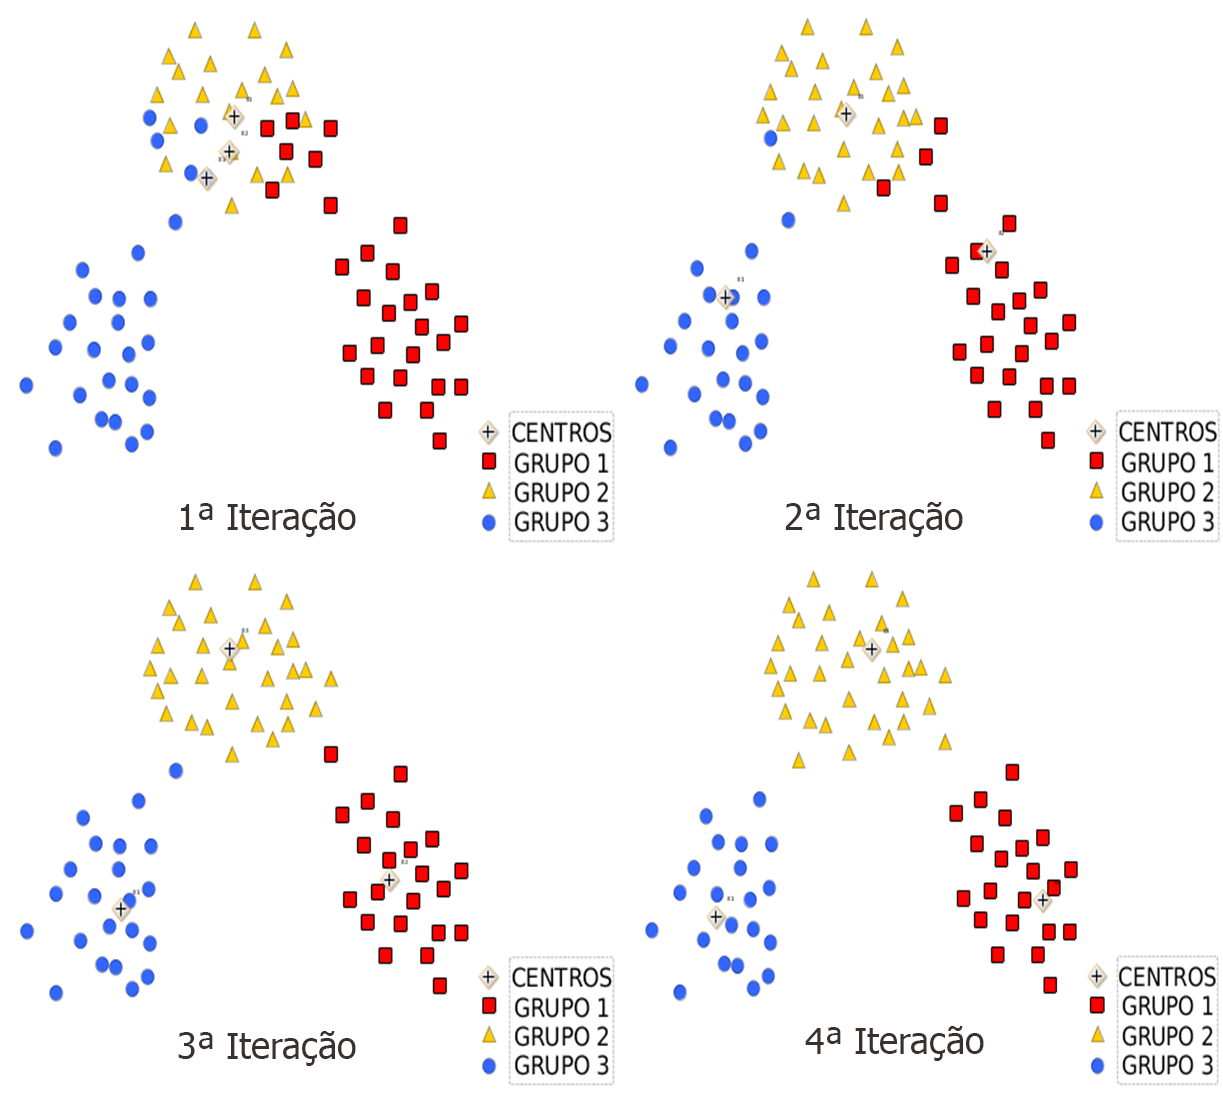
\includegraphics[width = 15cm, height = 13cm]{figuras/kmeans.png}
\caption{\scriptsize{Iterações do K-means.}}
\end{figure}

\indent Na Figura 1 são exemplificadas iterações do processo de clusterização. Na primeira iteração os centroides são atribuídos próximo ao centro dos dados. Então, os centroides são recalculados e os pontos são agrupados a cada próxima iteração, movendo-se em direção ao centros dos grupos. Quando não há mais alterações possíveis em relação aos centros, o K-means termina sua execução, pois os centroides já identificaram os agrupamentos. 

\indent Para calcular as distâncias entre os centroides e os elementos ainda dispersos, geralmente é utilizada função de distância Euclideana, que irá calcular a similaridade entre dois pontos, podendo ser definida na equação (2.1):

\begin{equation} 
\label{eq:Distância Euclidiana} %Título da equacao
\sqrt{(p_{x} - q_{x})^{2}} = \textbar p_{x} - q_{x} \textbar 
\end{equation}

\noindent onde o ponto $P = (p_{x})$ e o centroide $Q = (q_{x})$.

\indent Um problema na utilização do método de clusterização K-means é definir um número inicial e  apropriado de clusters para o agrupamento dos dados. Esta questão deve ser analisada de acordo com os pressupostos apresentados e com o tipo de dados que serão agrupados. Na detecção de anomalias em redes, a clusterização necessita de uma análise heurística realizada a partir de uma fase de treinamento, onde devem ser analisados os resultados da clusterização com quantidades diferentes de grupos (MÜNZ et al., 2007).

\indent Outro problema recorrente do K-means é referente a sua inicialização, caso alguns dos centroides sejam iniciados em pontos próximos, o k-means tende a estacionar estes pontos. O mesmo ocorre quando os centroides são iniciados em um mesmo grupo denso. Quando os pontos são inciados em locais distantes dos grupos o algoritmo tende a concentrar os centroides nos grupos mais populosos e o melhor desempenho de clusterização ocorre quando os objetos centrais são inciados no grupo menos populoso (ADANIYA, 2012).

\indent Algumas variações do K-means também estão presentes na literatura, o algoritmo K-medoids, se difere do K-means ao se constituir primeiramente na escolha de um objeto central, denominado \textit{medoid}. Ao final de uma iteração, onde os elementos são alocados aos grupos, o \textit{medoid} é substituído por outro elemento contido no grupo e não por uma média do elementos, como é feito no K-means. Outra variante é o algoritmo de Expectativa Maximização \textit{clustering} (EM), que primeiramente calcula a probabilidade de de cada objeto em relação a cada grupo e, em seguida, agrupa os dados nos grupos de maior probabilidade. O processo é repetido e os parâmetros de cada objeto são ajustados durantes as iterações até que se alcance a estabilidade (SYARIF et al., 2012). 

  \section{Trabalhos Relacionados}

\indent Diversos trabalhos de pesquisa analisam o problema da detecção de anomalias que estão relacionados com a proposta deste trabalho. Esta seção irá discutir alguns trabalhos relevantes, suas propostas, metodologias e os resultados obtidos.

\indent ULISSE (ZANERO, 2008) é um sistema de detecção de anomalias não supervisionado baseado em aprendizagem, desenvolvido em uma arquitetura de duas camadas. O algoritmo SOM (\textit{Self Organizing Map}) atua na primeira camada realizando o agrupamento dos pacotes de rede através do cálculo da distância euclidiana. Na segunda camada são realizadas verificações nos cabeçalhos dos pacotes, relacionando os dados das anomalias identificadas. O sistema apresenta bons resultados, além disso, possui ajustes de sensibilidade que aumentam as taxas de detecções, apresentando quantidades insignificantes de falsos positivos.

\indent O trabalho de Mazel et al (2015) utiliza uma metodologia que combina a análise de séries temporais e técnicas de agrupamento. O sistema produzido realiza análises no fluxo de dados da rede, ao encontrar mudanças na média de variância do fluxo, o sistema captura a série de tempo responsável pela variação. Para analisar a ocorrência de anomalias, é utilizado o algoritmo de agrupamento espacial baseado em densidade de aplicações com ruído (DBSCAN) que não necessita de informações prévias em relação à quantidade de grupos, como ocorre no K-means. Além disso, o sistema cria um \textit{ranking} das anomalias detectadas que mais estão prejudicando a rede. A taxa de falsos positivos identificados neste trabalho é inferior a um porcento das anomalias detectadas e o sistema foi capaz de detectar noventa e cinco porcento das anomalias do tráfego.

\indent Uma metologia supervisionada é proposta no trabalho de Wang et al (2008), que realiza o treinamento do sistema com clusterização do tráfego levando em consideração um grupo de tráfego normal e um grupo anômalo. Após a coleta das assinaturas com o agrupamento, o sistema compara as assinaturas com tráfego analisado através do cálculo da distância de Mahalanobis, enquadrando os eventos em um dos grupos. Apesar de eficiente, esta metodologia não consegue detectar anomalias ocasionadas somente por uma origem e um destino. O método também é aplicado ao correio eletrônico, verificando e-mails normais e anormais. 

\indent No trabalho de SYARIF et al (2012) é desenvolvido um estudo relacionado ao desempenho dos principais algoritmos de \textit{clustering} presentes na literatura em relação a detecção de anomalias no tráfego de rede. Na pesquisa, em uma mesma base de dados são aplicados os algoritmos K-means, K-medoids e Expectativa Maximização, onde os três algoritmos são superiores na detecção de anomalias desconhecidas em relação aos métodos baseados em mau uso. Mesmo quando não são utilizadas técnicas para o aperfeiçoamento, como, por exemplo, o treinamento ou as assinaturas do tráfego, os algoritmos de clusterização apresentam boas taxas de detecção.

\indent Uma combinação do K-means e árvores de decisão é proposta no trabalho de MINUYANDI et al (2012). O método utiliza primeiramente o K-means para o agrupamento dos dados e em cada grupo criado é aplicada a árvore de decisão C4.5 que irá refinar os limites dos dados normais e anormais em cada grupo. Os resultados mostram que o método é eficiente na detecção de anomalias, e as taxas de detecção são superiores a todos algoritmos com que foram comparados no trabalho.

\chapter{Desenvolvimento}

  \section{Bases de Dados}
\indent A base de dados de rede conhecida como DARPA foi criada pelo Lincoln Laboratory do Instituto Tecnológico de Massachusetts para avaliação de sistemas de detecção de intrusão e consequentemente é utilizado para detecção de anomalias. Na DARPA estão contidos dados de tráfego gerado a partir de uma mistura de máquinas reais e máquinas simuladas, onde o tráfego de fundo foi gerado artificialmente por estas máquinas e os ataques foram realizados contra as máquinas reais. Apesar da incerteza em relação a naturalidade do tráfego gerado artificialmente, esta base de dados é utilizada em grande escala na literatura.

\indent Dois cenários de ataques são simulados na DARPA o LLDOS 1.0 e o LLDOS 2.0. O primeiro cenário simula um atacante não muito experiente, que deixa clara sua presença na rede e no segundo cenário é simulado um atacante experiente que não deixa clara a sua presença na rede. Os ataques gerados nos dois cenários se baseiam em scanner de portas, ataques de negação de serviços e instalação de worms na rede.



  \section{Implementação}
  
  \section{Resultados}
  
\chapter{Conclusões}

  
%%Colocar as referências conforme as normas da ABNT, somente as utilizadas no trabalho e presentes neste manuscrito.

\begin{thebibliography}{99}

\bibitem{MONOWAR et al:2014}
{ABNTEX2; ARAUJO, L. C. \textbf{A classe abntex2}: Documentos técnicos e científicos brasileiros compatíveis com as normas ABNT. Sine loco, v. 1.9.2; 2014.}.

\bibitem{Biazin:2008}
{BIAZIN, D. T. \textbf{Normas da ABNT e padronização de trabalhos acadêmicos}. Londrina: Instituto Filadélfia de Londrina; 2008.}

\bibitem{Buneman:2011}
{BUNEMAN, P.; CHENEY, J.; LINDLEY, S. et al. \textbf{DBWiki}: A Structured Wiki for Curated Data and Collaborative Data Management. Athens: SIGMOD’11; 2011.}

\bibitem{Wikibooks:2014}
{WIKIBOOKS. \textbf{LaTeX}: The Free Textbook Project. Disponível em: <http://en.wikibooks.org/wiki/LaTeX>. Acesso em: 09 abr. 2014.}

\bibitem{ABNTEX2:2014}
{ABNTEX2; ARAUJO, L. C. \textbf{A classe abntex2}: Documentos técnicos e científicos brasileiros compatíveis com as normas ABNT. Sine loco, v. 1.9.2; 2014.}.

\bibitem{ABNTEX2:2014}
{ABNTEX2; ARAUJO, L. C. \textbf{A classe abntex2}: Documentos técnicos e científicos brasileiros compatíveis com as normas ABNT. Sine loco, v. 1.9.2; 2014.}.

\bibitem{ABNTEX2:2014}
{ABNTEX2; ARAUJO, L. C. \textbf{A classe abntex2}: Documentos técnicos e científicos brasileiros compatíveis com as normas ABNT. Sine loco, v. 1.9.2; 2014.}.

\bibitem{ABNTEX2:2014}
{ABNTEX2; ARAUJO, L. C. \textbf{A classe abntex2}: Documentos técnicos e científicos brasileiros compatíveis com as normas ABNT. Sine loco, v. 1.9.2; 2014.}.

\bibitem{ABNTEX2:2014}
{ABNTEX2; ARAUJO, L. C. \textbf{A classe abntex2}: Documentos técnicos e científicos brasileiros compatíveis com as normas ABNT. Sine loco, v. 1.9.2; 2014.}.

\end{thebibliography}

\end{document}
